\documentclass[aspectratio=169,handout]{beamer}
\usepackage{array}
\usepackage{libertine}
\usepackage{graphicx}
\usepackage{eurosym}
\usepackage{tikz}
\usepackage[T1]{fontenc}
\usepackage[utf8]{inputenc}

\renewcommand*\familydefault{\sfdefault}

\setbeamertemplate{navigation symbols}{}
\setbeamercolor{background canvas}{bg=white}
\setbeamercolor{title}{fg=black}
\setbeamercolor{titlelike}{fg=black}
\setbeamercolor{normal text}{fg=white!20!black}
\setbeamercolor{alerted text}{fg=normal text.fg}
\setbeamercolor{itemize item}{fg=gray}
\setbeamercolor{enumerate item}{fg=gray}
\setbeamercolor{description item}{fg=normal text.fg}
\setbeamerfont{alerted text}{family=\bf}
\setbeamerfont{description item}{family=\bf}
\usefonttheme[onlymath]{serif}

\usetikzlibrary{positioning}
\usetikzlibrary{datavisualization}
\usetikzlibrary{datavisualization.formats.functions}
\usetikzlibrary{shapes.geometric}
\usetikzlibrary{decorations.pathmorphing}

\def\doctolibLogo{img/doctolib_black}

\setbeamertemplate{footline} {\large \hspace{1ex}\insertframenumber/\inserttotalframenumber\vspace{1ex}}
\begin{document}
\title{Building a “native” Windows daemon with Node.JS}
\subtitle{}
\author{Victor Schubert <v@schu.be>}
\date{2020--02--04}

\frame{\titlepage}

\begin{frame}
	\frametitle{Who am I?}

	// I’m a fullstack developer at Doctolib GmbH; my team focuses on making
	sure our online doctor appointment booking service is interoperable with
	doctors’ specialized software.
\end{frame}

\begin{frame}
	\frametitle{Our peculiar use case}

	\begin{itemize}
		\item Show a screenshot of Doctolib with a quick presentation of what it does.
		\item Show a screenshot of some PMS with a quick presentation of what it does.
		\item Zipper in the middle runs on the doctors’ machine and synchronizes those.
	\end{itemize}
\end{frame}

\begin{frame}
	\frametitle{Let’s get things in order}

	\centering
	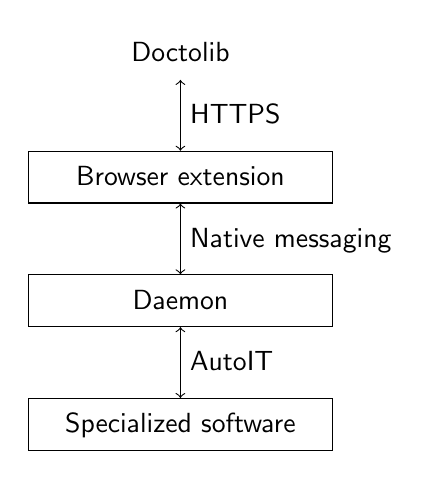
\begin{tikzpicture}[node distance=0.9,text height=.90em,text depth=.30em]
		\node (inet) [rectangle]                 {Doctolib};
		\node (flar) [minimum width=11em,draw,rectangle,below=of inet] {Browser extension};
		\node (rora) [minimum width=11em,draw,rectangle,below=of flar] {Daemon};
		\node (psql) [minimum width=11em,draw,rectangle,below=of rora] {Specialized software};
		\draw (inet) edge[<->] node[anchor=west] {HTTPS} (flar);
		\draw (flar) edge[<->] node[anchor=west] {Native messaging} (rora);
		\draw (rora) edge[<->] node[anchor=west] {AutoIT} (psql);
	\end{tikzpicture}
\end{frame}

\begin{frame}
	\frametitle{Web extensions, a primer}

	\begin{itemize}
		\item Written with standard browser Javascript.
		\item Now largely portable across browsers.
		\item {\em Very} sandboxed.
		\item Can communicate with local processes with {\em Native messaging}.
	\end{itemize}
\end{frame}

\begin{frame}
	\frametitle{Native messaging?}

	\begin{itemize}
		\item The browser spawns and manages a process.
		\item It sends messages through the process’ standard input.
		\item It receives messages from the process’ standard output.
		\item Messages use a JSON-based protocol.
		\item Not harder than \texttt{postMessage}.
	\end{itemize}
\end{frame}

\begin{frame}
	\frametitle{The Zipper daemon}

	\begin{itemize}
		\item Receives messages from the web extension.
		\item Takes action upon receiving these messages.
		\item Sends back messages with info and results.
		\item Directly reads files.
		\item Simulates user input on neighbouring software using AutoIT.
	\end{itemize}
\end{frame}

\begin{frame}
	\frametitle{What’s AutoIT?}

	\begin{itemize}
		\item Scripting language for GUI automation.
		\item It is also a library!
		\item But a DLL library.
		\item There’s a basic binding, but not sufficient.
	\end{itemize}
\end{frame}

\begin{frame}
	\frametitle{A picture speaks a thousand words}

	// Demo of AutoIT automation. Perhaps an OPEN\_PATIENT? Or just an AutoIT
	promotional video would suffice.
\end{frame}

\begin{frame}
	\frametitle{What’s a DLL again?}

	\begin{itemize}
		\item A {\em Dynamic Link Library}, duh…
		\item Contains code and data to be loaded and run by a program at runtime.
		\item Code and data are indexed by symbols.
		\item That’s not very different from how CommonJS imports work.
	\end{itemize}
\end{frame}

\begin{frame}
	\frametitle{DLLs aren’t too different from CommonJS modules actually}

	\begin{columns}
	\begin{column}{0.5\textwidth}
		A DLL…

		\begin{itemize}
			\item Has a symbol table.
			\item String keys in the symbol table point to functions and variables.
			\item Is loaded and cached/memoized by the OS.
		\end{itemize}
	\end{column}
	\begin{column}{0.5\textwidth}
		A CommonJS module…

		\begin{itemize}
			\item Has an \texttt{exports} object.
			\item String keys in the \texttt{exports} object reference functions and variables.
			\item Is loaded and cached/memoized by Node.JS.
		\end{itemize}
	\end{column}
	\end{columns}
\end{frame}

\begin{frame}
	\frametitle{So how do we call that native function?}

	You can use either ffi or N-API. \vspace{1em}

	\begin{columns}[t]
		\begin{column}{0.5\textwidth}
			ffi…
			\begin{itemize}
				\item Is a Node.JS module.
				\item Requires explicit code to load the library.
				\item Requires all types to be rewritten in Javascript.
				\item Can call all function synchronously or asynchronously.
			\end{itemize}
		\end{column}
		\begin{column}{0.5\textwidth}
			N-API…
			\begin{itemize}
				\item Is an API for building C++ libraries called from JS.
				\item Requires you to write bindings in C++.
				\item Requires all types to be specified in C++.
				\item Requires extra work to offer asynchronous and synchronous
					variants of functions.
			\end{itemize}
		\end{column}
	\end{columns}
\end{frame}

\begin{frame}
	\frametitle{So how do we call that native function with ffi?}

	// Code sample, maybe from Zipper Desktop so that we stay on-topic? Or a
	livecoding session. This can be demonstrated rather quickly with a dummy C
	library.
\end{frame}

\begin{frame}
	\frametitle{What when the DLL isn’t thread-safe?}

	That’s a topic for an entire talk, or maybe a blog post, such as this one!

	https://medium.com/doctolib/calling-into-thread-unsafe-dlls-with-node-ffi-1ef83806a50c

	// Add a QR-Code to the article.
\end{frame}

\begin{frame}
	\frametitle{So how is it all deployed?}

	\begin{itemize}
		\item It is all bundled as a single binary using Zeit’s PKG.
		\item PKG straps all of your code onto a modified Node.JS binary, to form
			a single file.
		\item Our daemon has custom logic to update itself.
		\item You can use Zeit to easily deploy a web server with all of its
			assets.
	\end{itemize}
\end{frame}

\begin{frame}
	\frametitle{Doctolib is recruiting!}

	\centering

	https://careers.doctolib.de/

	// Add a QR-Code.
\end{frame}

\begin{frame}
	\frametitle{Where to find me?}

	\centering

	\begin{tabular}{>{\bfseries}rl}
		\hspace{0.5\textwidth}&\hspace{0.5\textwidth}\\
		Name & Victor Schubert \\
		E-mail & v@schu.be \\
		Personal Github & schubev \\
		Company Github & doctolib \\
	\end{tabular}

	\vspace{1em}
	// Add a QR-Code and link to my own website. There I will also host the
	slides.
\end{frame}

\end{document}
% vim: set ts=3 sts=3 noet syntax=tex:
